% Generated by Sphinx.
\def\sphinxdocclass{report}
\documentclass[letterpaper,10pt,english]{sphinxmanual}
\usepackage[utf8]{inputenc}
\DeclareUnicodeCharacter{00A0}{\nobreakspace}
\usepackage[T1]{fontenc}
\usepackage{babel}
\usepackage{times}
\usepackage[Bjarne]{fncychap}
\usepackage{longtable}
\usepackage{sphinx}
\usepackage{multirow}
\setcounter{secnumdepth}{4}
\usepackage{fancyhdr}
%\usepackage{palatino}
\setcounter{tocdepth}{4}
\usepackage{fontspec}
\usepackage{xunicode}
\usepackage{xltxtra}
\setmainfont[Mapping=tex-text]{Birka}
\setsansfont{Myriad Roman}
\setmonofont{Inconsolata}
\makeatletter
  \fancypagestyle{normal}{
    \fancyhf{}
    \fancyfoot[LE,RO]{{\py@HeaderFamily\thepage}}
    \fancyfoot[LO]{{\py@HeaderFamily\nouppercase{\rightmark}}}
    \fancyfoot[RE]{{\py@HeaderFamily\nouppercase{\leftmark}}}
    \fancyhead[LE,RO]{{\py@HeaderFamily \@title}} % here's the change
    \renewcommand{\headrulewidth}{0.4pt}
    \renewcommand{\footrulewidth}{0.4pt}
  }
\makeatother
\textwidth 15truecm
\textheight 22.5truecm
\baselineskip 14truept
\oddsidemargin 1cm
\evensidemargin 1cm
\topmargin 0cm
\definecolor{VerbatimBorderColor}{rgb}{0.36,0.54,0.66}


\title{Low Level Design Documentation}
\date{October 06, 2012}
\release{0.1}
\author{Shiv Shankar Dayal \& Pavan Sharma}
\newcommand{\sphinxlogo}{}
\renewcommand{\releasename}{Release}
\makeindex

\makeatletter
\def\PYG@reset{\let\PYG@it=\relax \let\PYG@bf=\relax%
    \let\PYG@ul=\relax \let\PYG@tc=\relax%
    \let\PYG@bc=\relax \let\PYG@ff=\relax}
\def\PYG@tok#1{\csname PYG@tok@#1\endcsname}
\def\PYG@toks#1+{\ifx\relax#1\empty\else%
    \PYG@tok{#1}\expandafter\PYG@toks\fi}
\def\PYG@do#1{\PYG@bc{\PYG@tc{\PYG@ul{%
    \PYG@it{\PYG@bf{\PYG@ff{#1}}}}}}}
\def\PYG#1#2{\PYG@reset\PYG@toks#1+\relax+\PYG@do{#2}}

\def\PYG@tok@gd{\def\PYG@tc##1{\textcolor[rgb]{0.63,0.00,0.00}{##1}}}
\def\PYG@tok@gu{\let\PYG@bf=\textbf\def\PYG@tc##1{\textcolor[rgb]{0.50,0.00,0.50}{##1}}}
\def\PYG@tok@gt{\def\PYG@tc##1{\textcolor[rgb]{0.00,0.25,0.82}{##1}}}
\def\PYG@tok@gs{\let\PYG@bf=\textbf}
\def\PYG@tok@gr{\def\PYG@tc##1{\textcolor[rgb]{1.00,0.00,0.00}{##1}}}
\def\PYG@tok@cm{\let\PYG@it=\textit\def\PYG@tc##1{\textcolor[rgb]{0.25,0.50,0.56}{##1}}}
\def\PYG@tok@vg{\def\PYG@tc##1{\textcolor[rgb]{0.73,0.38,0.84}{##1}}}
\def\PYG@tok@m{\def\PYG@tc##1{\textcolor[rgb]{0.13,0.50,0.31}{##1}}}
\def\PYG@tok@mh{\def\PYG@tc##1{\textcolor[rgb]{0.13,0.50,0.31}{##1}}}
\def\PYG@tok@cs{\def\PYG@tc##1{\textcolor[rgb]{0.25,0.50,0.56}{##1}}\def\PYG@bc##1{\colorbox[rgb]{1.00,0.94,0.94}{##1}}}
\def\PYG@tok@ge{\let\PYG@it=\textit}
\def\PYG@tok@vc{\def\PYG@tc##1{\textcolor[rgb]{0.73,0.38,0.84}{##1}}}
\def\PYG@tok@il{\def\PYG@tc##1{\textcolor[rgb]{0.13,0.50,0.31}{##1}}}
\def\PYG@tok@go{\def\PYG@tc##1{\textcolor[rgb]{0.19,0.19,0.19}{##1}}}
\def\PYG@tok@cp{\def\PYG@tc##1{\textcolor[rgb]{0.00,0.44,0.13}{##1}}}
\def\PYG@tok@gi{\def\PYG@tc##1{\textcolor[rgb]{0.00,0.63,0.00}{##1}}}
\def\PYG@tok@gh{\let\PYG@bf=\textbf\def\PYG@tc##1{\textcolor[rgb]{0.00,0.00,0.50}{##1}}}
\def\PYG@tok@ni{\let\PYG@bf=\textbf\def\PYG@tc##1{\textcolor[rgb]{0.84,0.33,0.22}{##1}}}
\def\PYG@tok@nl{\let\PYG@bf=\textbf\def\PYG@tc##1{\textcolor[rgb]{0.00,0.13,0.44}{##1}}}
\def\PYG@tok@nn{\let\PYG@bf=\textbf\def\PYG@tc##1{\textcolor[rgb]{0.05,0.52,0.71}{##1}}}
\def\PYG@tok@no{\def\PYG@tc##1{\textcolor[rgb]{0.38,0.68,0.84}{##1}}}
\def\PYG@tok@na{\def\PYG@tc##1{\textcolor[rgb]{0.25,0.44,0.63}{##1}}}
\def\PYG@tok@nb{\def\PYG@tc##1{\textcolor[rgb]{0.00,0.44,0.13}{##1}}}
\def\PYG@tok@nc{\let\PYG@bf=\textbf\def\PYG@tc##1{\textcolor[rgb]{0.05,0.52,0.71}{##1}}}
\def\PYG@tok@nd{\let\PYG@bf=\textbf\def\PYG@tc##1{\textcolor[rgb]{0.33,0.33,0.33}{##1}}}
\def\PYG@tok@ne{\def\PYG@tc##1{\textcolor[rgb]{0.00,0.44,0.13}{##1}}}
\def\PYG@tok@nf{\def\PYG@tc##1{\textcolor[rgb]{0.02,0.16,0.49}{##1}}}
\def\PYG@tok@si{\let\PYG@it=\textit\def\PYG@tc##1{\textcolor[rgb]{0.44,0.63,0.82}{##1}}}
\def\PYG@tok@s2{\def\PYG@tc##1{\textcolor[rgb]{0.25,0.44,0.63}{##1}}}
\def\PYG@tok@vi{\def\PYG@tc##1{\textcolor[rgb]{0.73,0.38,0.84}{##1}}}
\def\PYG@tok@nt{\let\PYG@bf=\textbf\def\PYG@tc##1{\textcolor[rgb]{0.02,0.16,0.45}{##1}}}
\def\PYG@tok@nv{\def\PYG@tc##1{\textcolor[rgb]{0.73,0.38,0.84}{##1}}}
\def\PYG@tok@s1{\def\PYG@tc##1{\textcolor[rgb]{0.25,0.44,0.63}{##1}}}
\def\PYG@tok@gp{\let\PYG@bf=\textbf\def\PYG@tc##1{\textcolor[rgb]{0.78,0.36,0.04}{##1}}}
\def\PYG@tok@sh{\def\PYG@tc##1{\textcolor[rgb]{0.25,0.44,0.63}{##1}}}
\def\PYG@tok@ow{\let\PYG@bf=\textbf\def\PYG@tc##1{\textcolor[rgb]{0.00,0.44,0.13}{##1}}}
\def\PYG@tok@sx{\def\PYG@tc##1{\textcolor[rgb]{0.78,0.36,0.04}{##1}}}
\def\PYG@tok@bp{\def\PYG@tc##1{\textcolor[rgb]{0.00,0.44,0.13}{##1}}}
\def\PYG@tok@c1{\let\PYG@it=\textit\def\PYG@tc##1{\textcolor[rgb]{0.25,0.50,0.56}{##1}}}
\def\PYG@tok@kc{\let\PYG@bf=\textbf\def\PYG@tc##1{\textcolor[rgb]{0.00,0.44,0.13}{##1}}}
\def\PYG@tok@c{\let\PYG@it=\textit\def\PYG@tc##1{\textcolor[rgb]{0.25,0.50,0.56}{##1}}}
\def\PYG@tok@mf{\def\PYG@tc##1{\textcolor[rgb]{0.13,0.50,0.31}{##1}}}
\def\PYG@tok@err{\def\PYG@bc##1{\fcolorbox[rgb]{1.00,0.00,0.00}{1,1,1}{##1}}}
\def\PYG@tok@kd{\let\PYG@bf=\textbf\def\PYG@tc##1{\textcolor[rgb]{0.00,0.44,0.13}{##1}}}
\def\PYG@tok@ss{\def\PYG@tc##1{\textcolor[rgb]{0.32,0.47,0.09}{##1}}}
\def\PYG@tok@sr{\def\PYG@tc##1{\textcolor[rgb]{0.14,0.33,0.53}{##1}}}
\def\PYG@tok@mo{\def\PYG@tc##1{\textcolor[rgb]{0.13,0.50,0.31}{##1}}}
\def\PYG@tok@mi{\def\PYG@tc##1{\textcolor[rgb]{0.13,0.50,0.31}{##1}}}
\def\PYG@tok@kn{\let\PYG@bf=\textbf\def\PYG@tc##1{\textcolor[rgb]{0.00,0.44,0.13}{##1}}}
\def\PYG@tok@o{\def\PYG@tc##1{\textcolor[rgb]{0.40,0.40,0.40}{##1}}}
\def\PYG@tok@kr{\let\PYG@bf=\textbf\def\PYG@tc##1{\textcolor[rgb]{0.00,0.44,0.13}{##1}}}
\def\PYG@tok@s{\def\PYG@tc##1{\textcolor[rgb]{0.25,0.44,0.63}{##1}}}
\def\PYG@tok@kp{\def\PYG@tc##1{\textcolor[rgb]{0.00,0.44,0.13}{##1}}}
\def\PYG@tok@w{\def\PYG@tc##1{\textcolor[rgb]{0.73,0.73,0.73}{##1}}}
\def\PYG@tok@kt{\def\PYG@tc##1{\textcolor[rgb]{0.56,0.13,0.00}{##1}}}
\def\PYG@tok@sc{\def\PYG@tc##1{\textcolor[rgb]{0.25,0.44,0.63}{##1}}}
\def\PYG@tok@sb{\def\PYG@tc##1{\textcolor[rgb]{0.25,0.44,0.63}{##1}}}
\def\PYG@tok@k{\let\PYG@bf=\textbf\def\PYG@tc##1{\textcolor[rgb]{0.00,0.44,0.13}{##1}}}
\def\PYG@tok@se{\let\PYG@bf=\textbf\def\PYG@tc##1{\textcolor[rgb]{0.25,0.44,0.63}{##1}}}
\def\PYG@tok@sd{\let\PYG@it=\textit\def\PYG@tc##1{\textcolor[rgb]{0.25,0.44,0.63}{##1}}}

\def\PYGZbs{\char`\\}
\def\PYGZus{\char`\_}
\def\PYGZob{\char`\{}
\def\PYGZcb{\char`\}}
\def\PYGZca{\char`\^}
\def\PYGZsh{\char`\#}
\def\PYGZpc{\char`\%}
\def\PYGZdl{\char`\$}
\def\PYGZti{\char`\~}
% for compatibility with earlier versions
\def\PYGZat{@}
\def\PYGZlb{[}
\def\PYGZrb{]}
\makeatother

\begin{document}

\maketitle
\tableofcontents
\phantomsection\label{index::doc}


Contents:


\chapter{Introduction}
\label{intro:introduction}\label{intro::doc}\label{intro:welcome-to-low-level-design-s-documentation}
This document describes the low level design of libreQA Q\&A platform. Libraries
used are CppCMS, and Mimetic. We also use Google, Facebook, Linkedin and Twitter
jQuery APIs. The entire pages are sent as JSON data from server which is rendered
in browser using jQuery. Some AJAX pre-loading is done to improve the
responsiveness of application. We will use jQuery Javsscript framework. No HTML or
CSS is directly written. Database used is MongoDB. Programming language used is
C++ for server side and DB access. We will use CMake as build system and Kdevelop
as our primary IDE. GNU/Linux 64-bit system will be used for development.
Repository is located at \href{https://github.com/shivshankardayal/libreqa.git}{https://github.com/shivshankardayal/libreqa.git}
Coding standards of CppCMS will be used for this development. Later we will use
OpenMP and OpenMPI for parallel processing and distributed computing.
For Mathematics we will use MathJAX and for syntax highlighting we will use
syntax highlighter with TinyMCE.

Given below are the world wide web uris for these:
\begin{enumerate}
\item {} 
\href{http://cppcms.com/}{http://cppcms.com/}

\item {} 
\href{http://www.mongodb.org/}{http://www.mongodb.org/}

\item {} 
\href{http://www.codesink.org/mimetic\_mime\_library.html}{http://www.codesink.org/mimetic\_mime\_library.html}

\item {} 
\href{http://jquery.com/}{http://jquery.com/}

\item {} 
\href{http://www.tinymce.com/}{http://www.tinymce.com/}

\item {} 
\href{http://www.mathjax.org/}{http://www.mathjax.org/}

\item {} 
\href{https://github.com/efloti/plugin-mathjax-pour-tinymce}{https://github.com/efloti/plugin-mathjax-pour-tinymce}

\item {} 
\href{https://github.com/RichGuk/syntaxhl}{https://github.com/RichGuk/syntaxhl}

\end{enumerate}


\chapter{Architecture}
\label{arch::doc}\label{arch:architecture}
It is assumed that standard MongoDB sharding will be used as shown (the
image was shamelessly copied from \href{http://www.mongodb.org}{http://www.mongodb.org} ) below:

{\hfill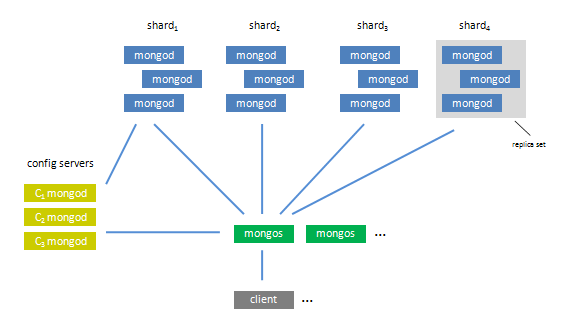
\includegraphics{sharding.PNG}\hfill}

User can hit MongoDB's website to know about it.


\section{Models}
\label{arch:models}

\subsection{Questions \& Answers}
\label{arch:questions-answers}
Folowing model(read collection) is in picture for questions and answers:

\begin{Verbatim}[commandchars=\\\{\}]
\PYGZob{}
        Questions : \PYGZob{}
                Question no. : Long Long,
                title        : String,
                Body             : html,
                tags             : Sorted List of Strings,
                view             : Integer,
                votes            : Integer,
                favorite         : Inetger,
                timestamp        : Timestamp,
                Followers        : List of users,
                Comments         :List of comments \PYGZob{}
                        comment    : String,
                        timestamp  : TimeStamp,
                        commeneter : user,
                \PYGZcb{},
                answers : List of answers \PYGZob{}
                        Answer id : Long Long,
                        answer    : String,
                        accepted  : Boolean,
                        votes     : Integer,
                        Comments  : List of comments \PYGZob{}
                                comment    : String,
                                timestamp  : TimeStamp,
                                commeneter : user,
                        \PYGZcb{},
                \PYGZcb{},
        \PYGZcb{},
\PYGZcb{}
\end{Verbatim}

Following model(read collection) is for users:

\begin{Verbatim}[commandchars=\\\{\}]
\PYGZob{}
        Users: \PYGZob{}
                Name              : String,
                Email id          : String,
                URL                       : String,
                Date of Birth : Date,
                Karma             : Long Long,
                Skills            : Tags,
                Badges            : List of Badges \PYGZob{}
                        Badge Name        : Name,
                        Date Acquired : Date,
                \PYGZcb{},
                Questions : List of Questions Asked \PYGZob{}
                        Question URL : String,
                \PYGZcb{},
                Answers : List of Answers Given \PYGZob{}
                        Question URL with answer ref: URL,
                \PYGZcb{}
        \PYGZcb{}
\PYGZcb{}
\end{Verbatim}

Following collection is for tags:

\begin{Verbatim}[commandchars=\\\{\}]
\PYGZob{}
        Tags : \PYGZob{}
                Name : String,
                Count : Integer,
                links : List of question for that tag \PYGZob{}
                        link: URL
                \PYGZcb{}
        \PYGZcb{}
\PYGZcb{}
\end{Verbatim}

Following collection is for badges:

\begin{Verbatim}[commandchars=\\\{\}]
\PYGZob{}
        Badges : \PYGZob{}
                Users : List of people having that badge,
                Count : Long Long,
        \PYGZcb{}
\PYGZcb{}
\end{Verbatim}


\chapter{Indices and tables}
\label{index:indices-and-tables}\begin{itemize}
\item {} 
\emph{genindex}

\end{itemize}



\renewcommand{\indexname}{Index}
\printindex
\end{document}
